\subsubsection{ソフトウェア設計の文脈}

ソフトウェア設計は、開発ライフサイクルの中で孤立して存在しない。要求、アーキテクチャ、実装、テスト、保守と強くつながっている。

\begin{itemize}
  \item \textbf{要求との関係}：要求は、設計が解くべき問題を示す。設計は、要求を実装可能な構造と振る舞いへ変換する。
  \item \textbf{アーキテクチャとの関係}：アーキテクチャが定められている場合、それは設計の制約となる。主要構成要素、接続、API、採用すべきスタイルやパターン、設計原則などを制約する。
  \item \textbf{実装との関係}：設計は、実装者が何を作るべきかを示す案内である。実装者がコードを読む前に、部品の責務やインタフェースを理解できることが望ましい。
  \item \textbf{テストとの関係}：設計は、テスト戦略とテストケースの土台になる。設計要素が要求をどう満たすかが明らかであれば、テストの観点も作りやすい。
\end{itemize}

設計の形式性は、プロジェクトによって異なる。安全性が重要なシステムでは、設計記述を厳密に残す必要がある。一方、小規模な探索的開発では、簡潔なモデルやコードそのものが設計記録の中心になる場合もある。ただし、どの場合でも、関係者が設計判断を理解できることが重要である。

\begin{figure}[htbp]
\centering
\IfFileExists{assets/generated_figures/ch03/fig-ch03-03.png}{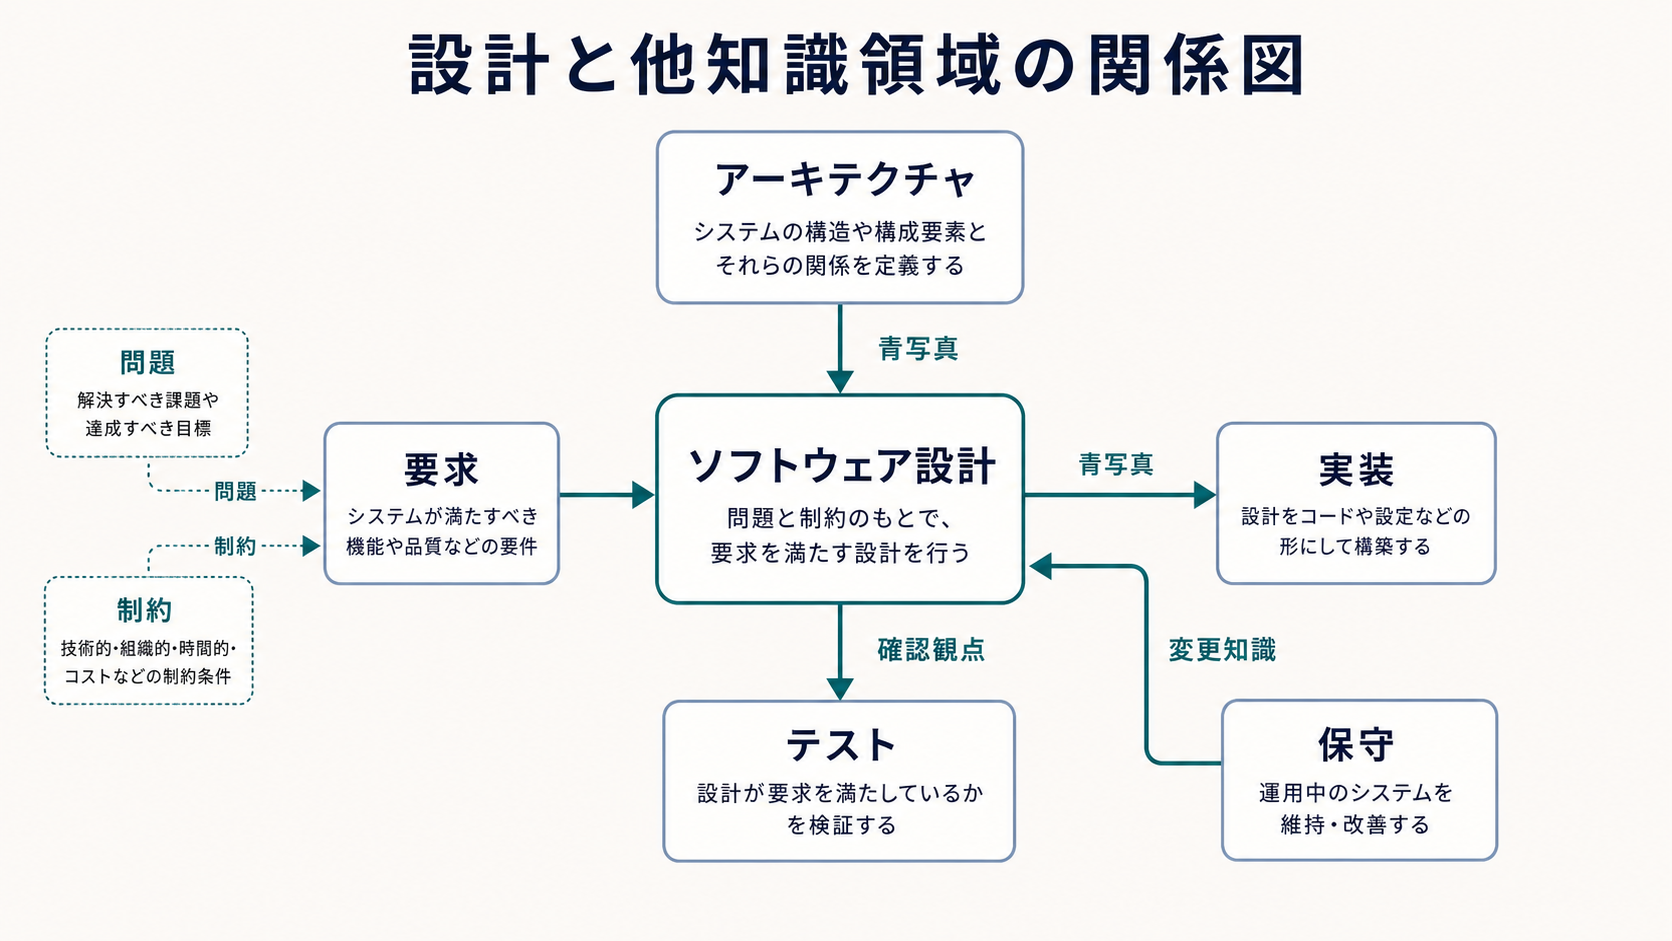
\includegraphics[width=0.96\linewidth]{assets/generated_figures/ch03/fig-ch03-03.png}}{\fbox{\parbox[c][48mm][c]{0.9\linewidth}{\centering 画像生成待ち\\設計と他知識領域の関係図}}}
\caption{設計と他知識領域の関係図}
\label{fig:ch03-03}
\end{figure}
